\documentclass[british]{article}

\usepackage[british]{babel}% Recommended
\usepackage{csquotes}% Recommended

\usepackage[sorting=nyt,style=apa]{biblatex}

\addbibresource{~/Tex/library.bib}

\usepackage[margin=1in]{geometry}
\usepackage{appendix}
\usepackage{amsmath}
\usepackage{graphicx}
\usepackage{listings}
\usepackage{enumerate}
\usepackage{color}
\newcommand{\code}[1]{\texttt{#1}}
\newtheorem{defin}{Definition}
\newtheorem{prop}{Proposition}
\newtheorem{col}{Corollary}
\newtheorem{thm}{Theorem}
\setlength{\parskip}{1em}
\usepackage{placeins}
\DeclareLanguageMapping{british}{british-apa}

\title{CS4402 Practical 2 - Binary constraint solver}
\author{170008773}
\date{\today}
\begin{document}
	\maketitle
	
	\section{Introduction}
	For this assignment, a basic binary constraint solver was to be implemented using Forward Checking (FC) and 2-way branching. The solver was also required to be able to use both dynamic and static heuristics.  Eventually, the solver was extended to utilise Maintaining Arc Consistency (MAC). An empirical comparison between the algorithms and several heuristics was also made. MAC with a dynamic, smallest domain heuristics performed best overall. 
	
	
	\section{Desing and implementation}
	\subsection{Variables and domains}
	\paragraph{Variables}To make some of the necessary bookkeeping easier, such as keeping track of the domains, a \code{CSPVariable} class was implemented. This class keeps track of things such as the domain, whether the variable is assigned, the name of the variable and eventually what order it has in a possible static heuristic. The name of the variable also enables naming variables instead of merely assigning them a numeric id, which is favourable when modelling more complex problems. 
	
	\paragraph{Domains} The domains were originally modelled as integer ranges but this was quickly changed to being modelled by a \code{Set} of integers. This was done for several reasons. Firstly this supports domains which are not continuous ranges, which is required for certain problems. Secondly, this allows for fast checking of containment, adding and removal of values which is instrumental for a constraint solver. Thirdly, this allows for easier extensions when more complex objects become desirable in domains. 
	
	\subsection{Constraints vs. Arcs} Since the solver only had to support binary table constraints the constraints are modelled as two variables and a set of tuples. The tuples representing the allowed value assignments, and stored in a list. This proved problematic for two reasons. Firstly there was the trouble of finding the correct constraints without having to check all of them since this would be very expensive for a large number of constraints. Secondly, it introduced a lot of ambiguity over the domain of which variable had to get pruned. This was eventually solved by two changes. Firstly the constraints were converted from bi-directional constraints into uni-directional arcs. So for example that meant that the constraint $c(x,y) = \{\langle1,2\rangle\}$ would be stored as $c(x,y) = \{\langle1,2\rangle\}$ \textit{and} $c(y,x) = \{\langle2,1\rangle\}$, with the implicit assumption that the second variable was always the one getting pruned. This allowed the constraints to be stored in a \code{Map<CSPVariable, Map<CSPVariable, BinaryArc>>}, meaning that we would index the arcs by the ``origin" and then by the ``destination" variable. This allowed for fast assessment of the relevant constraints and removed the ambiguity over which domain would have to be pruned, at the cost of extra storage space. It is important to note however that this does not imply extra work in the upkeep of the domains since support is bi-directional by definition. It also meant that \code{hashCode} and \code{equals} methods had to be written for all the classes in the containment chain, but this proved to be no problem. It also allowed for easy retrieval of all outgoing or incoming arcs, given a variable, which proved very useful in the implementation of MAC to be discussed later. 
	
	\subsubsection{Pruning} The solver also needed a mechanic to undo the pruning of domains that was done by the arc revision upon backtracking. Since FC nor MAC ever backtrack more than one level at a time, a \code{Stack} was chosen to record the most recent domain changes. That way, upon backtracking, only the top of the stack had to be restored. The changes were recorded by having the \code{revise} method simply return a \code{Set} of all values that were removed from the domain. These values were then stored in a \code{Map<CSPVariable, Set<Integer>>}  and then pushed onto the stack. Since \code{CSPVariable} already had its \code{hashCode} and \code{equals} methods implemented this was fairly simple. 
	
	\subsection{Heuristics}
	\subsubsection{Dynamic heuristics}
	To support the use of heuristics, a \code{PriorityQueue} was used to store the variables. The type of heuristics used was determined by which \code{Comparator}
	was used. Here a custom one was implemented for the dynamic smallest domain heuristic. This comparator simply checked the sizes of the domains of the two variables. It was chosen to make the dynamic smallest domain heuristic the default option. 
	\subsubsection{Static heuristics} The static heuristics were implemented in much the same way as the dynamic, with the added complexity that a file containing the order has to be supplied at runtime. The heuristic is then read in in the format of \code{name,order}, with each line containing exactly one pair, without any input checking, i.e. the reader assumes that all the variables in the problem are also present in the heuristic file. A Heuristic generator was also implemented, though the format of the heuristic files was designed to be readable and writable for both humans and machines. In the heuristic generator, code for generating the heuristics for llexographic and maximum degree variable ordering was also implemented. 
	
	When the static heuristic is used the order in which the variables are to be processed is stored within the variable class, which is technically a breach of abstractions. It does, however, make the code for storing and accessing the variables a lot simpler and more elegant, so this was deemed acceptable. Care was also taken to make sure that the variables could operate without these orderings so that the variables could still be used in other contexts. 
	
	\subsection{MAC}
	The only tangible difference between FC and MAC is the use of AC3. AC3 proved easy to implement after the arc model was introduced since this provided easy ways of accessing the correct arcs as mentioned previously. 
	
	\subsection{Testing}
	Testing was done through a variety of methods. Firstly, a solver using backtracking was also implemented to be able to generate the correct answers to small problems for comparison and to get a baseline for performance for the empirical evaluation. Secondly, the testing was mostly done with the use of \code{assert} statements to provide sanity checks where possible and make the program fail immediately upon violating one of these checks. This allowed easier diagnosis and ultimately faster debugging of the code, as well as confidence that the solutions produced were correct. Here \code{assert} statements were used not only to let the program fail as fast as possible but also to be able to easily disable the checking after the design was done since the checks done are not always trivial and can incur performance penalties. 
	
	\subsection{Design limitations and advantages} 
	\paragraph{Limitations}The design of the solver has a few flaws. Firstly, there is a lot of common code between the three solvers (one using backtracking, FC and MAC respectively). It would have been better to implement these using a basic abstract solver class and then providing mechanics to extend the common parts by way of inheritance and or interface implementation. This would have made the code more compact and easier to maintain. Secondly, not a lot of flexibility is offered to use different dynamic heuristics at the user level. The static heuristics can be altered by the user by manually editing the files, but no such mechanic exists for the dynamic heuristics. It would have been nice to provide some mechanic to the user to be able to use different dynamic heuristics. The solvers also do little to no input checking, which is obviously less than ideal. Finally, the statistics that the solvers keep track of are hard coded. It might have been nice to let the user either define or pick from several statistics to keep track of during runs. All of these functionalities, whoever, were deemed to be outside the scope of this project. 
	
	
	\section{Emperical evaluation}
	\subsection{Experiment setup}
	To collect the data for analysis a Python script was used. The solvers keep track of the number of arcs revised and branches explored during their runs. Note that the number of branches explored is not the same as the number of assignments made since 2-way branching was used. The python script will run all the solvers on all of the found problems with all the heuristics, which it will generate using the \code{HeuristicGenerator} class. It will then capture the output and write the statistics to a \code{.csv} file allowing for easier analysis. The script should be run as \code{`python runAllProblems.py`} and the code can be found in appendix \ref{collection}.
	
	\subsection{Results}
	
	\begin{figure}[!ht]
		\centering
		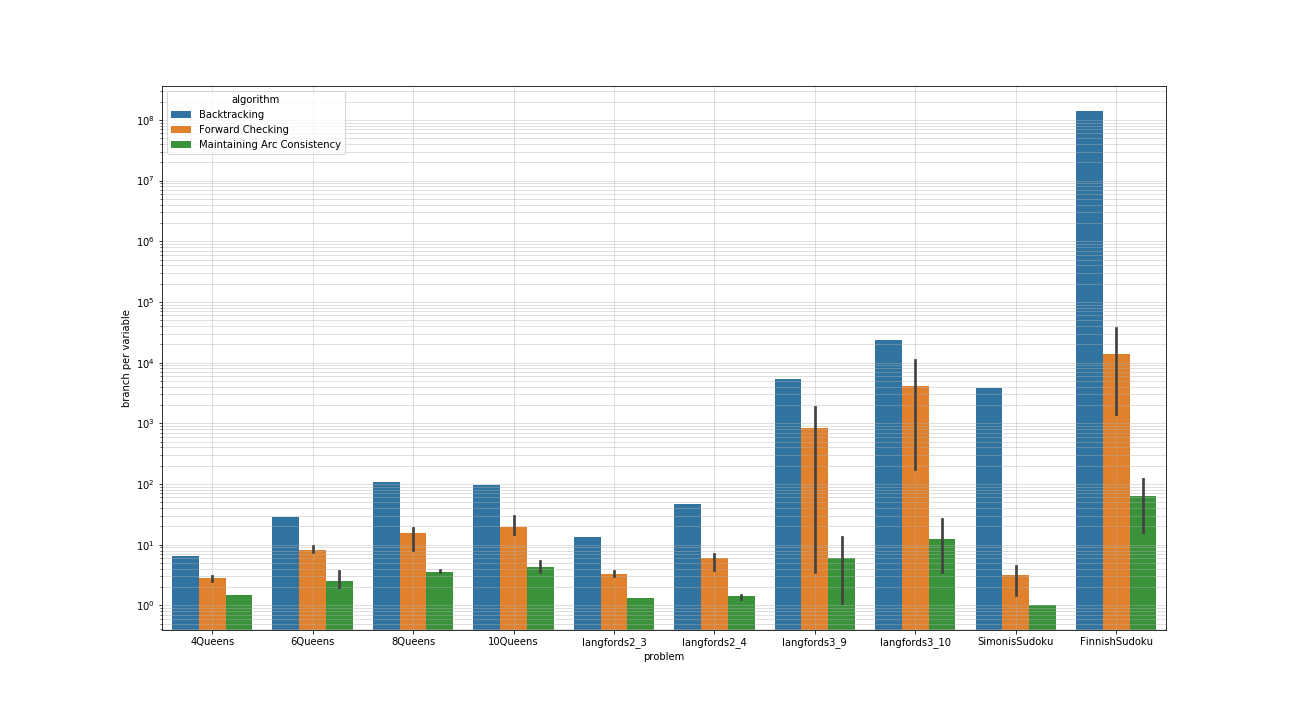
\includegraphics[width=0.9\textwidth]{meanBranchPerAlgo}
		\caption{A bargraph of the mean number of branches explored of every problem by algorithm. (lower is better)}
		\label{byAlgo}
	\end{figure}
	
	\begin{figure}[!ht]
		\centering
		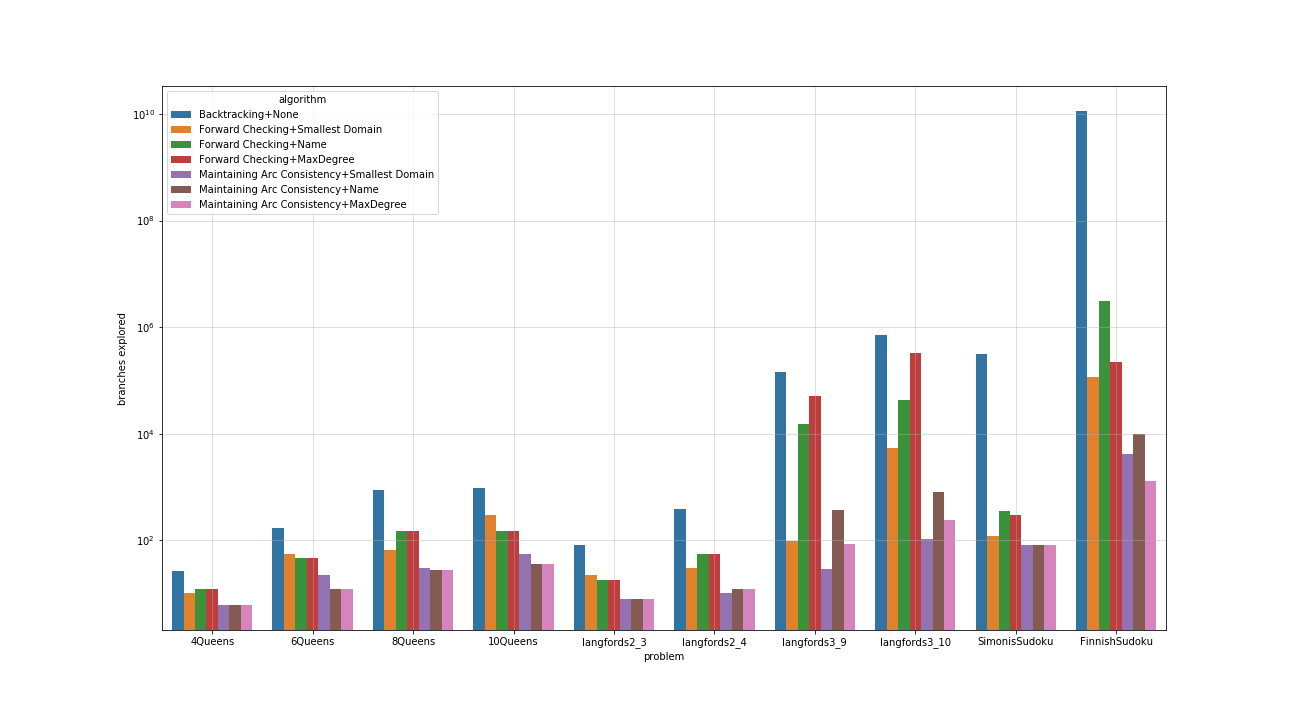
\includegraphics[width=0.9\textwidth]{branchPerAlgoAndHeuristic}
		\caption{A bargraph of the number of branches explored of every problem by algorithm and heuristic (lower is better)}
		\label{byHeuristic}
	\end{figure}
	
	\subsubsection{Algorithms}
	A bar graph depicting the average number of branches explored by each algorithm per problem averaged over the heuristics used can be found in figure \ref{byAlgo}. Here it easy to see that there exists a clear hierarchy. MAC outperforms FC which in term outperforms Backtracking, in all problems. This was what we expected to see since all of these algorithms are extensions of each other. It is interesting to note that the more constraints there are, the more gains each algorithm has over the previous version. This is again not surprising since that is what the extra work performed by each of the algorithms is for.
	
	
	\subsubsection{Heuristics}
	A more detailed look at the data can be found in figure \ref{byHeuristic}. Here the number of branches per algorithm and the individual heuristic is visualised. Here we see that in all the cases the dynamic heuristic performed best. In all cases, using FC with a less-than-optimal heuristic was still preferable to using backtracking. The Max Degree ordering usually performed either equally well as the lexicographical ordering, or worse. It should be noted that the performance of the Max Degree heuristic depends largely on how homogeneous the problem is. For example, the constraint graph of the N-Queens problem is essentially fully connected, so the Max Degree heuristic is essentially useless here (because of how the heuristic generator was implemented in this case it is equivalent to the lexicographical ordering). The Langfords problem, on the other hand, is quite different since the different variables have different degrees, and it is here that we see a difference in performance. One would suspect that the Max Degree ordering would have fared better here but that turned out not to be the case.  
	
	\section{Conclusion}
	\label{conclusion}
	In this report design and implementation details of the binary constraint solver have been discussed. An empirical evaluation of the three implemented solvers was also presented. Here it was seen that there was a clear hierarchy between the three solvers with MAC performing best. In all algorithms, the dynamic heuristic also performed best.
	
	word count: 1670
	\printbibliography
	
	\begin{appendices}
		\section{Experimental collection script}
		\label{collection}
		\lstinputlisting{../runAllProblems.py}
	\end{appendices}
	
	
\end{document}